\subsection{Ca sử dụng điền thông tin cơ bản}

Người dùng sau khi đăng ký hoặc thiếu thông tin sẽ thực hiện việc điều thông tin cơ bản. Sau khi hoàn thành 4 form thông tin, người dùng mới có thể sử dụng các tính năng khác của hệ thống.

Mô tả chi tiết cho ca sử dụng điền thông tin cơ bản được thể hiện ở Bảng \ref{tab:basic-info-usecase} dưới đây. Kèm theo là Bảng \ref{tab:basic-info-usecase-activity} về biểu đồ hoạt động, quan hệ và Hình \ref{fig:3-3-3-sequence-diagram} về biểu đồ tuần tự của ca sử dụng này. 

\noindent 
\begin{table}[H]
\centering
\begin{tabularx}{\linewidth}{| l | X |} 
\hline 
\textbf{Mô tả} & Người dùng cập nhật thông tin cá nhân như ngày sinh, tên, khảo sát, ảnh đại diện và thực hiện 1 số thao tác làm quen với tính năng hệ thống. \\ 
\hline 
\textbf{Luồng cơ bản} & 1. Người dùng đăng ký tài khoản mới. \newline
                       2. Người dùng tải ảnh đại diện lên. \newline
                       3. Người dùng điền tên và ngày sinh. \newline
                       4. Người dùng upload 3 ảnh lên để hệ thống hiển thị và giới thiệu tính năng gán nhãn ảnh. \newline
                       5. Người dùng điền form khảo sát. \newline
                       6. Người dùng bấm nút hoàn thành. \newline
                       7. Hệ thống điều hướng người dùng đến trang chủ của ứng dụng. \\
\hline 
\textbf{Luồng thay thế} &
                       - Nếu thông tin nhập vào không hợp lệ sẽ thông báo lỗi để người dùng nhập lại. \\ 
\hline 
\textbf{Tiền điều kiện} & Người dùng đăng ký tài khoản thành công và chưa hoàn thành điền hết 4 form thông tin cá nhân. \\
\hline 
\textbf{Hậu điều kiện} & - Thông tin cá nhân của người dùng được cập nhật. \newline
                       - Ảnh đại diện và 3 ảnh được upload lên sẽ được hệ thống đưa vào thư viện người dùng. \\ 
\hline 
\textbf{Yêu cầu phi chức năng} & Hệ thống xử lý gán nhãn ảnh không quá 5s \\
\hline 
\end{tabularx}
\caption{Mô tả chi tiết ca sử dụng điền thông tin cơ bản.}
\label{tab:basic-info-usecase}
\end{table}
\vspace{0.8cm}

\noindent
\begin{table}[H]
\centering
\begin{tabular}{| c | c |}
    \hline
    \textbf{Biểu đồ hoạt động} & \textbf{Quan hệ} \\ 
    \hline
    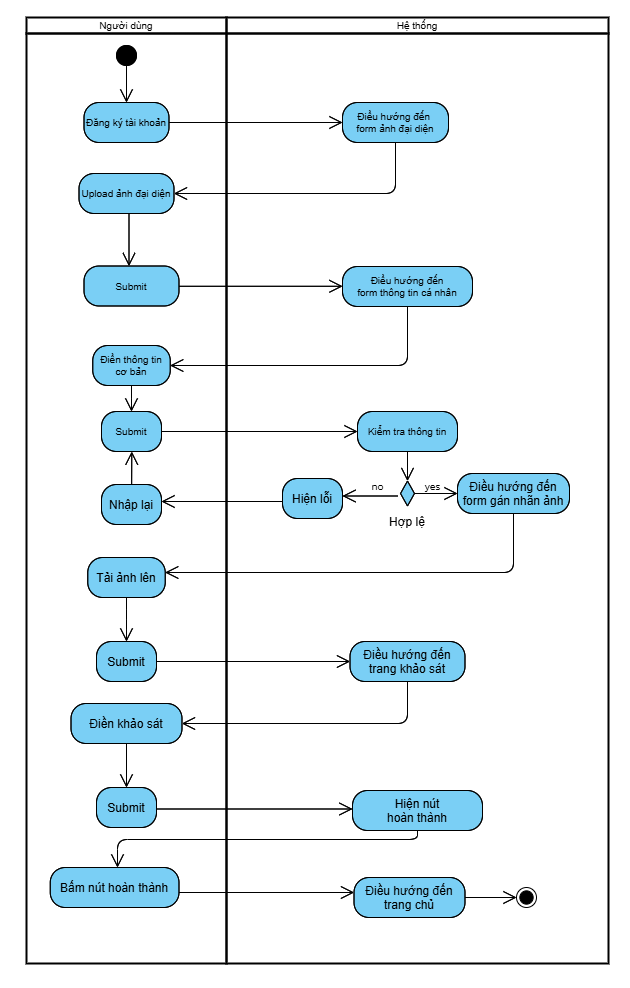
\includegraphics[width=0.6\linewidth]{figures/c3/3-3-3-activity-diagram.png} 
    & 
    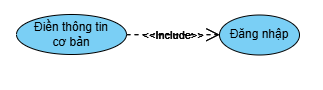
\includegraphics[width=0.35\linewidth]{figures/c3/3-3-3-relationship.png} \\ 
    \hline
\end{tabular}
\caption{Biểu đồ hoạt động và quan hệ ca sử dụng điền thông tin cơ bản.}
\label{tab:basic-info-usecase-activity}
\end{table}

\noindent
\begin{figure}[H]
    \centering  
    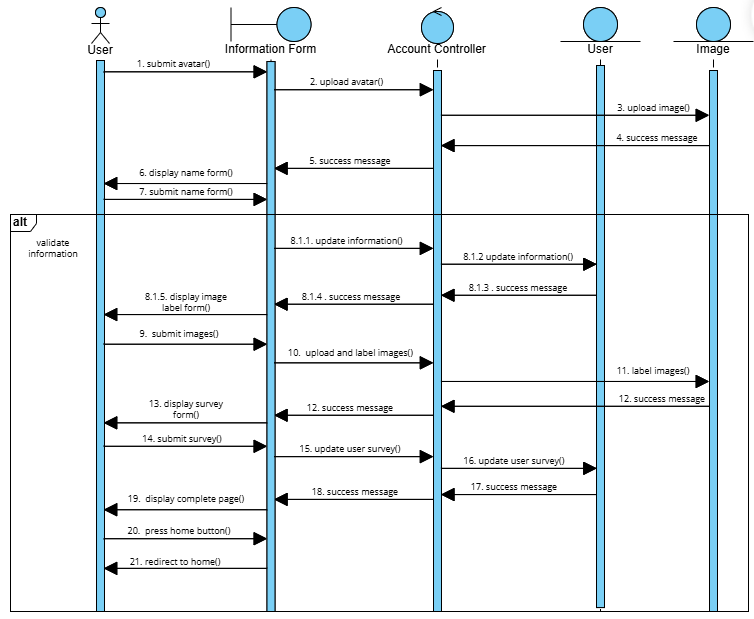
\includegraphics[width=1.1\textwidth]{figures/c3/3-3-3-sequence-diagram.png}
    \caption{Biểu đồ tuần tự ca sử dụng điền thông tin cơ bản.}
    \label{fig:3-3-3-sequence-diagram}
\end{figure}